% =====================================================================
\section{Additional theory and experiments}
\label{app:additional}

This appendix collects the detailed material omitted from the nine-page main text.
All reported numbers use the same checkpoints and seeds as the main comparison.

\subsection{Deferred theory statements}
\label{app:deferred-theory}

\begin{proposition}[Ambiguity--approximation decomposition]
\label{prop:pgib-ambiguity-decomposition}
For OPB classification with $\eta_k(x)=P(Y=k\mid X=x)$ and a comparator mean $h(x)$,
\begin{equation}
\mathcal K(w_0)=\frac{a^2}{2\tau^2}\E[1-\|\eta(X)\|_2^2]
+\frac1{2\tau^2}\E\left\|h(X)-a\sum_k\eta_k(X)q_{0,k}\right\|^2+V_0,
\label{eq:opb-ambiguity-decomposition}
\end{equation}
where $V_0$ is the covariance mismatch. For EPB regression,
\begin{equation}
\mathcal K(w_0)=\frac{\rho^2}{2\tau^2}\E[\operatorname{Var}(\tilde Y\mid X)]
+\frac1{2\tau^2}\E\|h(X)-\rho\nu(X)u_0\|^2+V_0.
\label{eq:epb-ambiguity-decomposition}
\end{equation}
\end{proposition}

Substituting either decomposition into $B_\beta$ in
Corollary~\ref{cor:pgib-beta-transfer} separates the comparator-dependent geometry
transfer floor into label ambiguity, encoder mean approximation, and covariance
mismatch.

\begin{corollary}[Zero-floor exact-realizability special cases]
\label{cor:pgib-exact-alignment}
Under deterministic labels, exact posterior--prior matching, and a compatible Bayes
head, $\mathcal K(w_0)=0$ and Theorem~\ref{prop:pgib-alignment} gives
\begin{equation}
\mathcal D(\widehat w)\le(\ln K+\varepsilon)/\beta
\label{eq:pgib-alignment}
\end{equation}
for classification. For EPB regression,
\begin{equation}
\mathcal D(\widehat w)\le(\tau^2/\rho^2+\varepsilon)/\beta.
\label{eq:pgib-alignment-regression}
\end{equation}
\end{corollary}

\begin{proposition}[Positive rate cost of class-independent means]
\label{prop:opb-collapse}
If $\E[\mu_\phi(X)\mid Y=k]=c$ for every class, then
\begin{equation}
\E\left[\frac{\|\mu_\phi(X)-a q_{\theta,Y}\|^2}{2\tau^2}\right]
\ge\frac{a^2}{2\tau^2}\left(1-\sum_k\pi_k^2\right).
\label{eq:opb-collapse}
\end{equation}
\end{proposition}

\begin{corollary}[The orthogonal instance instantiates conditional posterior separation]
\label{prop:opb-separation}
For OPB, $\tau_{\max}=\tau=1$ and $\Delta(y,y')=\sqrt2a$, so
\begin{equation}
\|m(y)-m(y')\|\ge\sqrt2a-\sqrt{2\tau^2D(y)}-\sqrt{2\tau^2D(y')}.
\label{eq:opb-separation}
\end{equation}
\end{corollary}

\subsection{Factor-wise ablations}
\label{app:ablation}
The factor-wise ablation ladder switches geometry, anchor scale, readout, and the IB
term separately; each variant is evaluated at its best validation-selected
configuration (Table~\ref{tab:ablation}). The complete means are reported in
Table~\ref{tab:ablation}. The paired bootstrap intervals are in the main text
(Table~\ref{tab:ablation-ci}) for the classification contrasts and in
Table~\ref{tab:ablation-ci-epb} for the regression mirrors; all paired differences
use the shared seeds at each variant's best validation-selected configuration,
and the intervals are $95\%$ bootstrap percentile CIs with $B=10{,}000$ and a fixed
seed. The factor ranking and
the sign-flip and negative-result patterns are read in the main text
(Section~\ref{sec:ablation}).

\emph{NCM-learn} removes the bottleneck entirely: the encoder output is used
deterministically ($z=\mu_\phi(x)$, no posterior and no KL) and classified by an
energy readout on trainable prototypes. \emph{NCM-ortho} is the same, except that
the prototypes are fixed to the orthogonal frame $a\,e_k$ (fixed geometry, still no
IB). \emph{CEB-energy} and \emph{CEB-tied} keep CEB's trainable free reference and
KL but replace its free head by the energy readout (resp.\ the tied projection).
\emph{OPB-FS} and \emph{EPB-FS} keep the orthogonal frame and the energy (resp.\
tied) readout but make the anchor radius learnable, so only the fixed scale is
switched off. \emph{EPB-L} and \emph{EPB} are the regression counterparts of GPB-L
and GPB on Housing, keeping the isometric-axis prior with a free head (resp.\ the
tied projection).

\begin{table}[t]
\centering
\small
\caption{Attribution ablation: best-configuration test metrics (mean $\pm$ std
over seeds). Configurations are selected by the mean validation metric
(accuracy on MNIST and ImageNet-100), applied identically to
every variant, so all comparisons remain paired by seed and the test split is
never touched by selection. One OPB-FS configuration (ImageNet-100,
$\beta = 10^{-4}$, $a = 1$) diverged during training (free scales grow without
penalty at negligible $\beta$) and is excluded.}
\label{tab:ablation}
\begin{tabular}{l c c}
\hline
variant & MNIST (Acc \%) & ImageNet-100 (Acc \%) \\
\hline
Base & $98.33 \pm 0.12$ & $83.12 \pm 0.14$ \\
NCM-learn & $98.17 \pm 0.17$ & $82.17 \pm 0.36$ \\
NCM-ortho & $98.11 \pm 0.12$ & $82.33 \pm 0.60$ \\
CEB & $98.43 \pm 0.08$ & $82.78 \pm 0.22$ \\
CEB-energy & $98.22 \pm 0.10$ & $81.59 \pm 0.21$ \\
GPB-L & $98.43 \pm 0.07$ & $83.40 \pm 0.67$ \\
GPB & $98.44 \pm 0.08$ & $84.22 \pm 0.15$ \\
OPB-RV & $98.34 \pm 0.04$ & $83.38 \pm 0.52$ \\
OPB-FS & $98.54 \pm 0.03$ & $84.26 \pm 0.18$ \\
\hline
\end{tabular}
\end{table}


\begin{table}[t]
\centering
\tiny
\begin{tabular}{l l c}
\hline
factor & comparison & Housing \\
\hline
readout (EPB) & EPB $-$ EPB-L & $-0.00$ [$_{-0.01}$, $_{-0.00}$] \\
geometry (EPB) & EPB-FS $-$ CEB-tied & $+0.01$ [$_{-0.00}$, $_{0.01}$] \\
fixed scale (EPB) & EPB $-$ EPB-FS & $+0.00$ [$_{-0.01}$, $_{0.01}$] \\
\hline
\end{tabular}
\caption{Regression mirrors of the factor-wise paired differences ($R^2$ on
Housing; $95\%$ bootstrap percentile CIs; positive values favor the first
term).}
\label{tab:ablation-ci-epb}
\end{table}

\subsection{Regression compression curves}
\label{app:compression}
The main text shows the classification compression sweep. This companion figure gives
the complete California Housing regression sweep under the same $\beta$ grid, including
the weak-compression variance explosion and the strong-compression EPB plateau. The
curves are diagnostics of achieved KL and task performance, not tests of the alignment
rate.

\begin{figure*}[t]
\centering
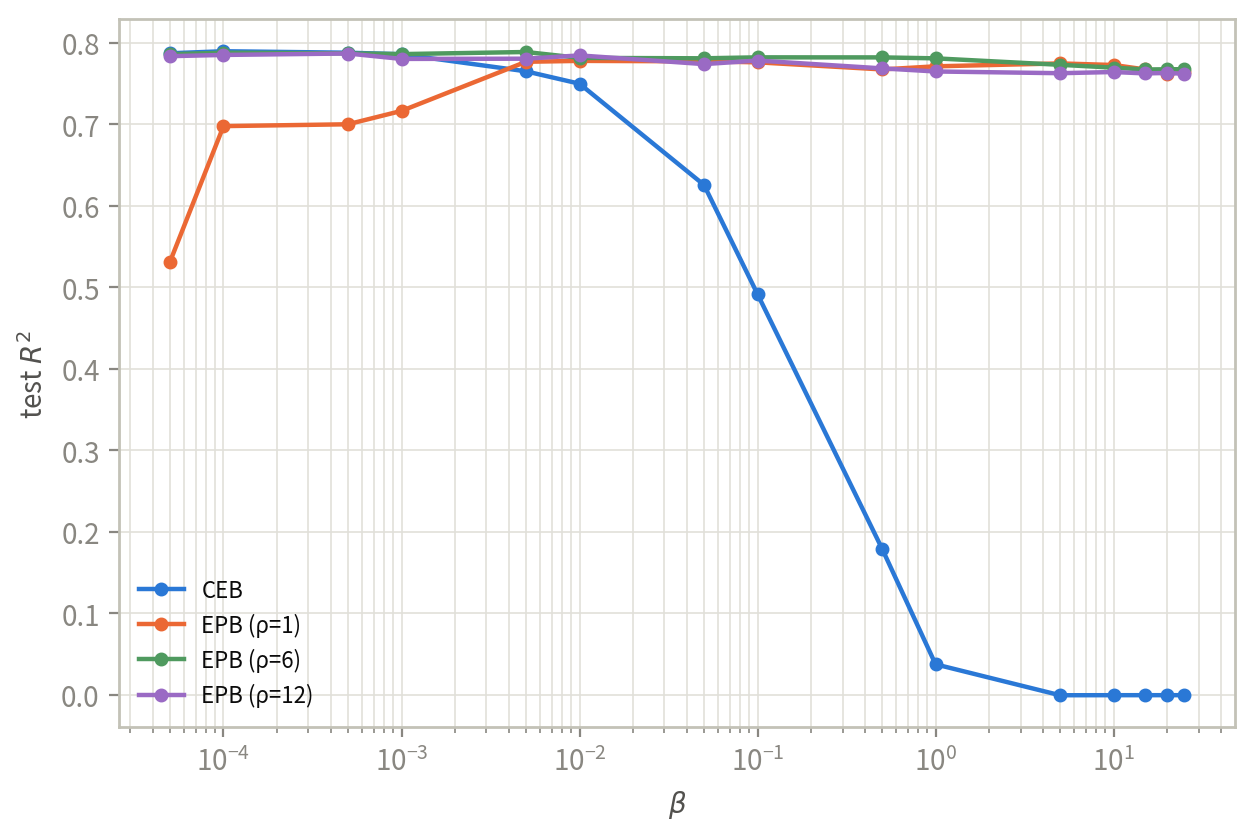
\includegraphics[width=0.48\linewidth]{figures/fig_beta_acc_housing.png}\hfill
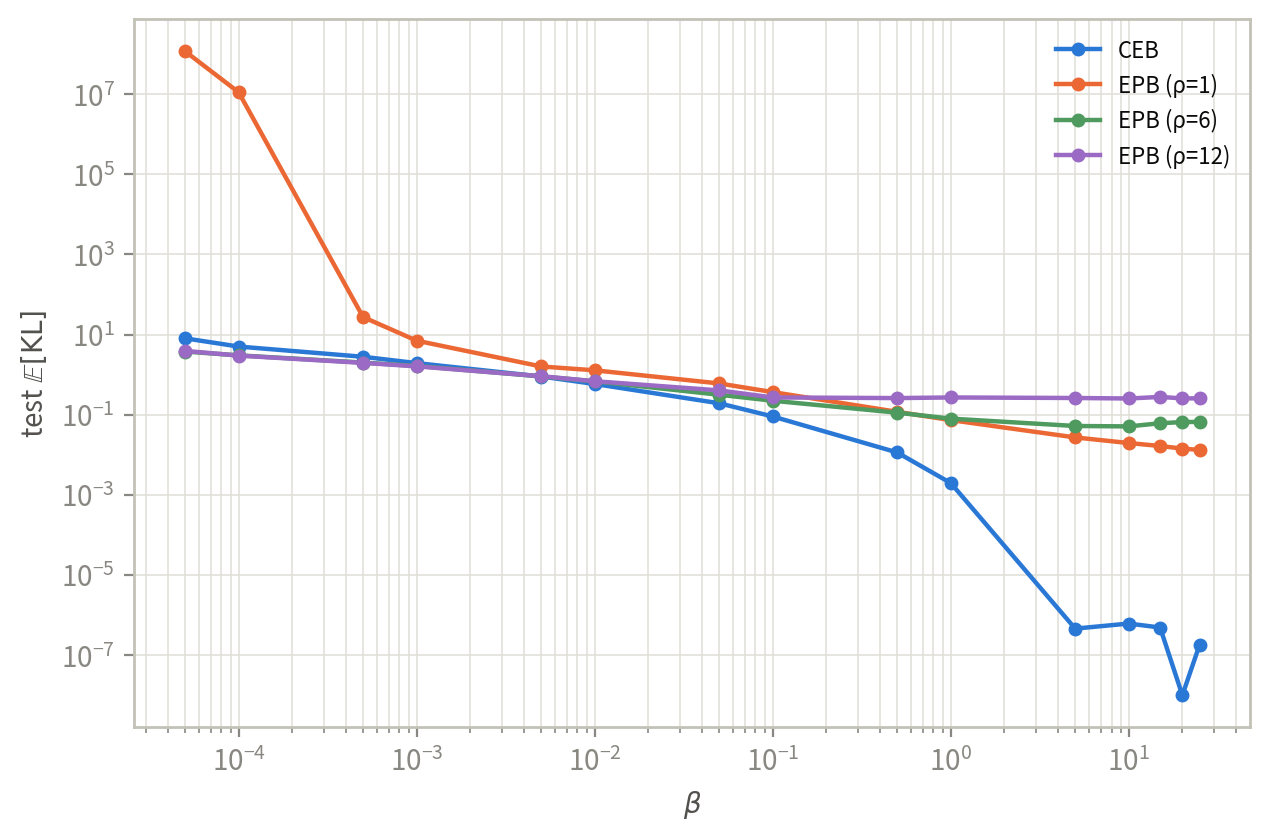
\includegraphics[width=0.48\linewidth]{figures/fig_beta_kl_housing.png}
\caption{California Housing compression sweep (MLP). Left: test $R^2$; right:
realized conditional KL over $\beta$. EPB maintains a task plateau through strong
compression, while the $\rho=1$ weak-compression points exhibit a large variance term.}
\label{fig:compression-housing}
\end{figure*}

\subsection{Anchor-scale sensitivity}
\label{app:scale-sensitivity}
The main comparison fixes the prior scale at $a=\rho=12$
(Sec.~\ref{sec:setup}); Fig.~\ref{fig:scale-sensitivity} reads the full
nine-point scale grid at weak, medium, and strong compression on the two
representative settings, complementing the $\beta$-axis
sweeps of Sec.~\ref{sec:sweep} with the scale-axis view.

\begin{figure*}[t]
\centering
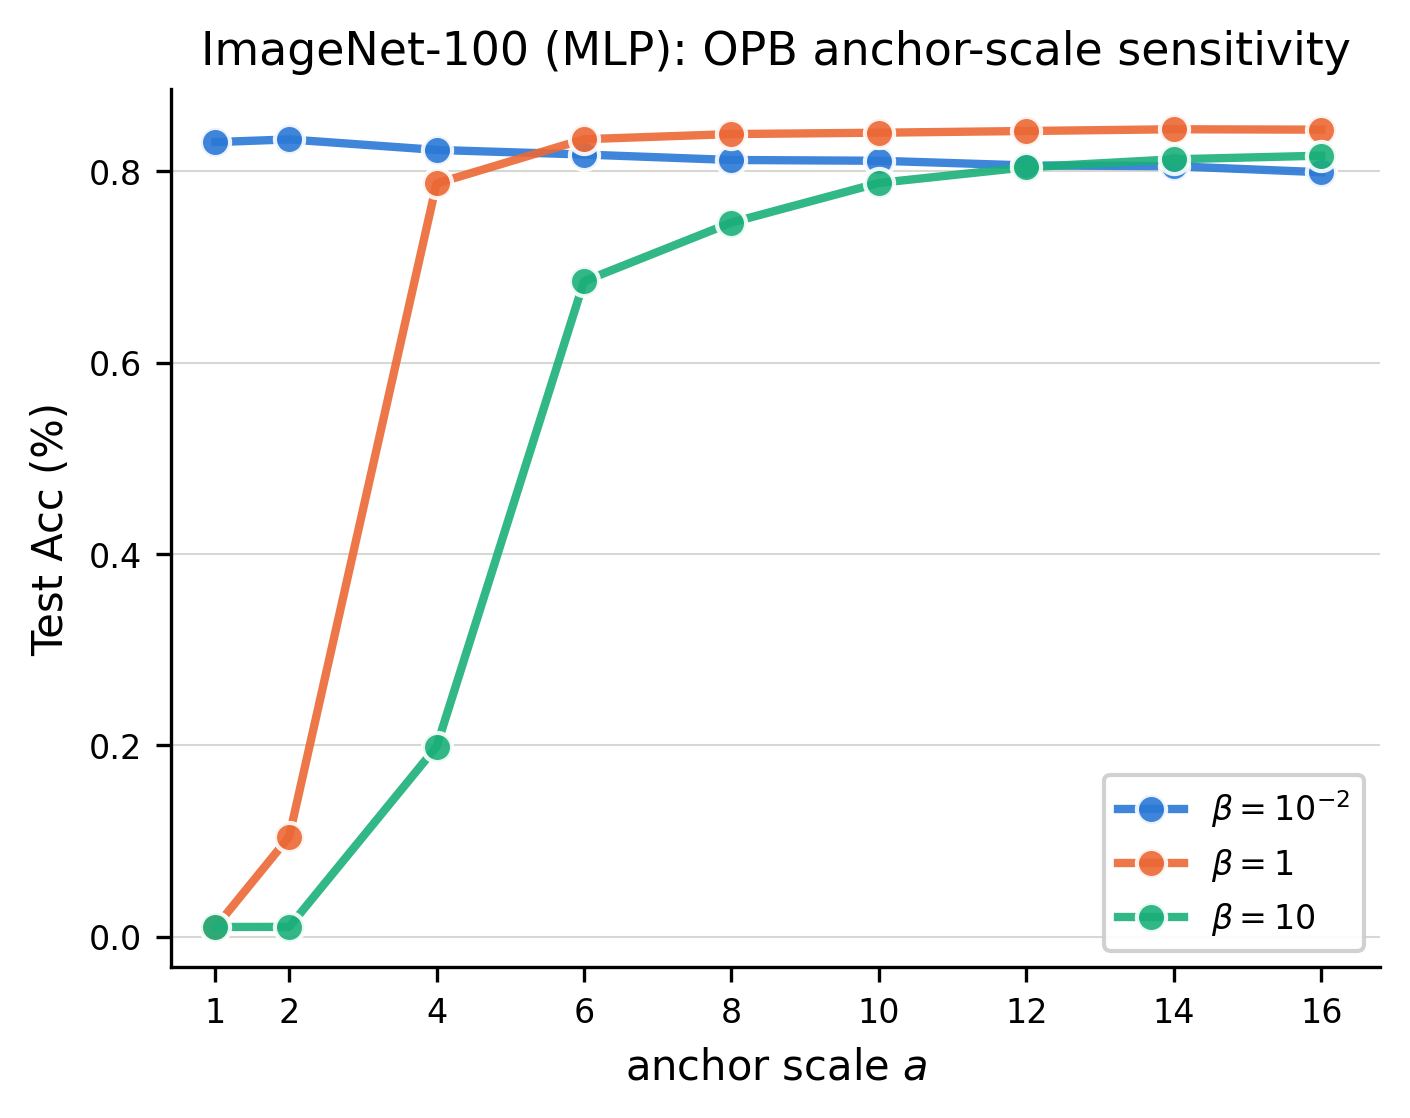
\includegraphics[width=0.49\linewidth]{figures/fig_anchor_sensitivity_imagenet100_mlp.png}\hfill
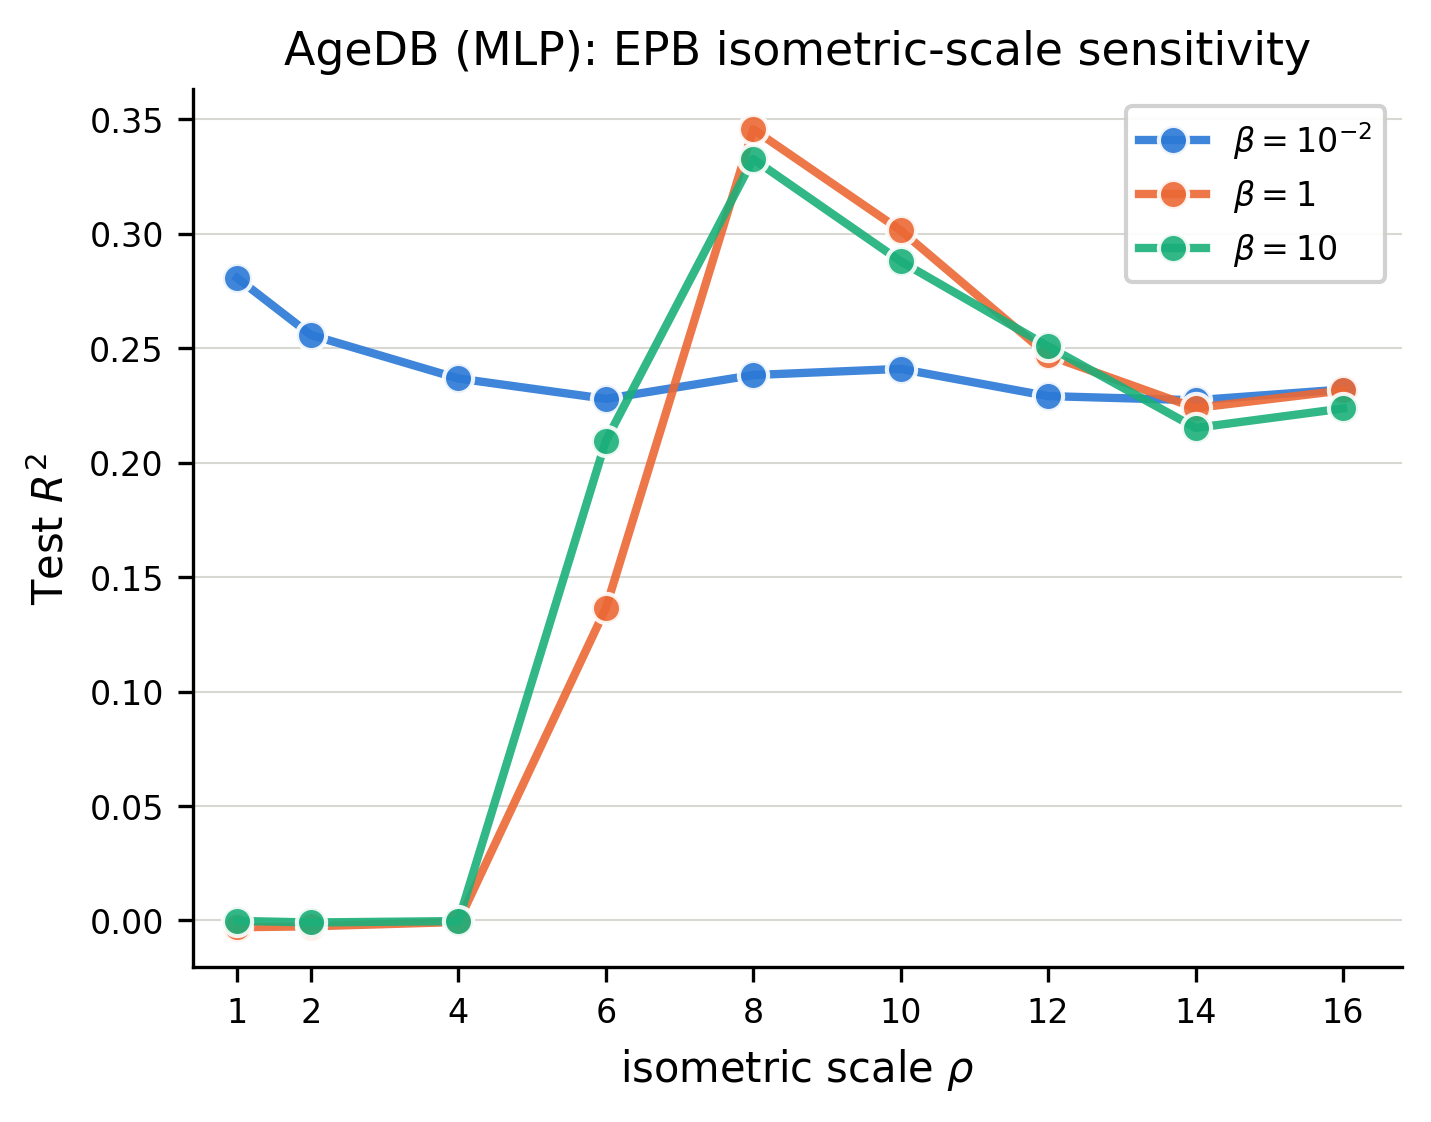
\includegraphics[width=0.49\linewidth]{figures/fig_anchor_sensitivity_agedb_mlp.png}
\caption{Anchor-scale sensitivity: (a) ImageNet-100 (MLP) OPB test accuracy
against the anchor scale $a$; (b) AgeDB (MLP) EPB test $R^2$ against the
isometric scale $\rho$; $\beta\in\{10^{-2},1,10\}$ (weak/medium/strong
compression).}
\label{fig:scale-sensitivity}
\end{figure*}

On both settings the scale matters only once compression bites: the
weak-compression curves are flat (within $3.4$ points on ImageNet-100),
and at $\beta\ge1$ scales below $4$ collapse (to chance accuracy on
ImageNet-100, to zero $R^2$ on AgeDB) while every scale above $6$ stays
on a plateau; the operating point is therefore sensitive to the scale
only through this collapse boundary, and the fixed $a=\rho=12$ lies
inside the retained band.

\subsection{Information-plane estimates}
\label{app:info-plane}
Estimator protocol.\ $I(X;Z)$ is estimated by the InfoNCE lower bound
\citep{oord2018representation} ($\log B-\mathcal{L}_{\mathrm{NCE}}$, $B=4096$; one
critic per run, trained on the training split, the bound read off the test split with
$z\sim q(z|x)$). $I(Y;Z)$ is read on the same sampled posterior: $H(Y)-\mathrm{CE}$
with the cross-entropy averaged over $M=20$ draws $z\sim q(z|x)$ per test point
(still a lower bound, as $\mathrm{CE}\ge H(Y|Z)$). The residual $I(X;Z|Y)$ is
estimated directly rather than as a difference: every $q(z|x)$ is a known Gaussian,
so the class-conditional mixture
$q(z|y)=\frac{1}{N_y}\sum_{j:y_j=y}q(z|x_j)$ over the test samples is evaluated
exactly by logsumexp, and
$I(X;Z|Y)=\mathbb{E}_{x,y}\,\mathrm{KL}(q(z|x)\,\|\,q(z|y))$ is read by Monte
Carlo---an exact estimate up to $z$-sampling noise and the finite per-class test
sample, not a difference of bounds. The certificate-plane axis is drawn linear
because the collapsed CEB trajectory lands on zero. The MNIST panels appear in
Fig.~\ref{fig:compression-main}(c,d) of the main text.

Matched-compression performance.
Table~\ref{tab:info-plane-matched} pairs each CEB point with the OPB configuration of
nearest estimated $I(X;Z)$. At $\approx2.0$ nat, CEB ($\beta=0.5$) retains $86.0\%$
while OPB ($a=1$, $\beta=0.5$) retains $97.8\%$; at $\approx2.5$ nat ($\beta=0.1$) the
two tie ($98.2\%$ vs.\ $98.1\%$). The directly estimated residual is comparable or
slightly larger for OPB at both points ($0.41$ vs.\ $0.47$ nat at $\beta=0.1$;
$0.20$ vs.\ $0.21$ nat at $\beta=0.5$), so OPB's task plateau is not bought by extra
residual compression. These are paired empirical comparisons at two estimated
compression levels, not a causal attribution to geometry.

\begin{table}[t]
\centering\small
\begin{tabular}{l c c c l c c c}
\hline
Setting & CEB $I(X;Z)$ & CEB $I(X;Z|Y)$ & CEB Acc. & OPB config. & OPB $I(X;Z)$ & OPB $I(X;Z|Y)$ & OPB Acc.\\
\hline
MNIST, $\beta=0.1$ & $2.54$ & $0.41$ & $98.2$ & $a=1,\beta=0.1$ & $2.55$ & $0.47$ & $98.1$\\
MNIST, $\beta=0.5$ & $1.96$ & $0.20$ & $86.0$ & $a=1,\beta=0.5$ & $2.01$ & $0.21$ & $97.8$\\
\hline
\end{tabular}
\caption{Matched-compression information-plane comparison (means; standard deviations
are in the stored evaluation report).}
\label{tab:info-plane-matched}
\end{table}

\subsection{Adversarial robustness details}
\label{app:robustness}
Targeted PGD uses 20 steps, EOT-10 gradients, 10-sample MC predictions, and budgets
$\varepsilon_\infty=0.3$ and $\varepsilon_2=6$. Curves are shown only when clean
stochastic accuracy exceeds $90\%$. At maximum compression, OPB $(a=6,12)$ reaches
$31.1\%/30.5\%$ targeted success under $L_\infty$, while transfer attacks from CEB
to OPB reach at most $2.0\%$/$3.4\%$ under $L_\infty/L_2$, far below OPB's white-box
attack. The transfer result is a gradient-masking check rather than a causal geometry
test.

\begin{figure*}[t]
\centering
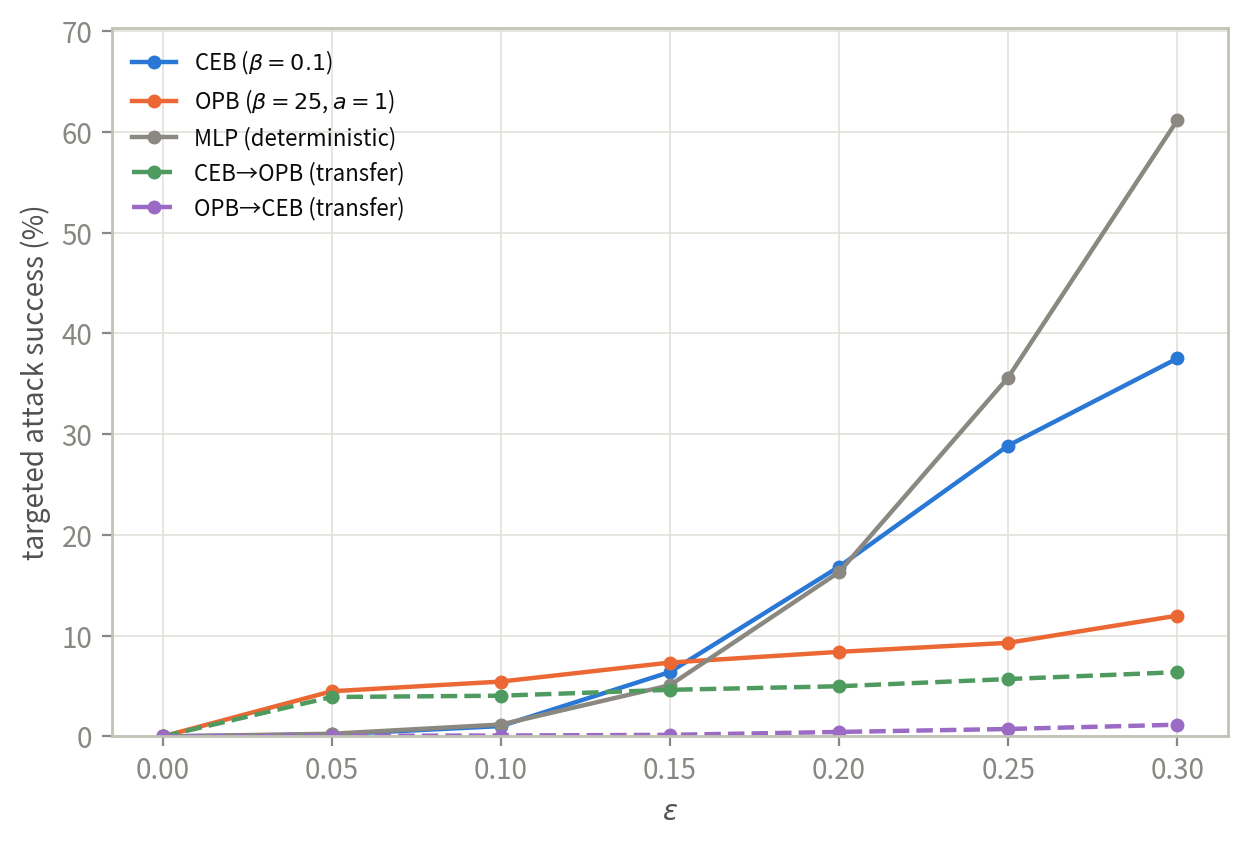
\includegraphics[width=0.48\linewidth]{figures/fig_adv_transfer_linf_mnist.png}\hfill
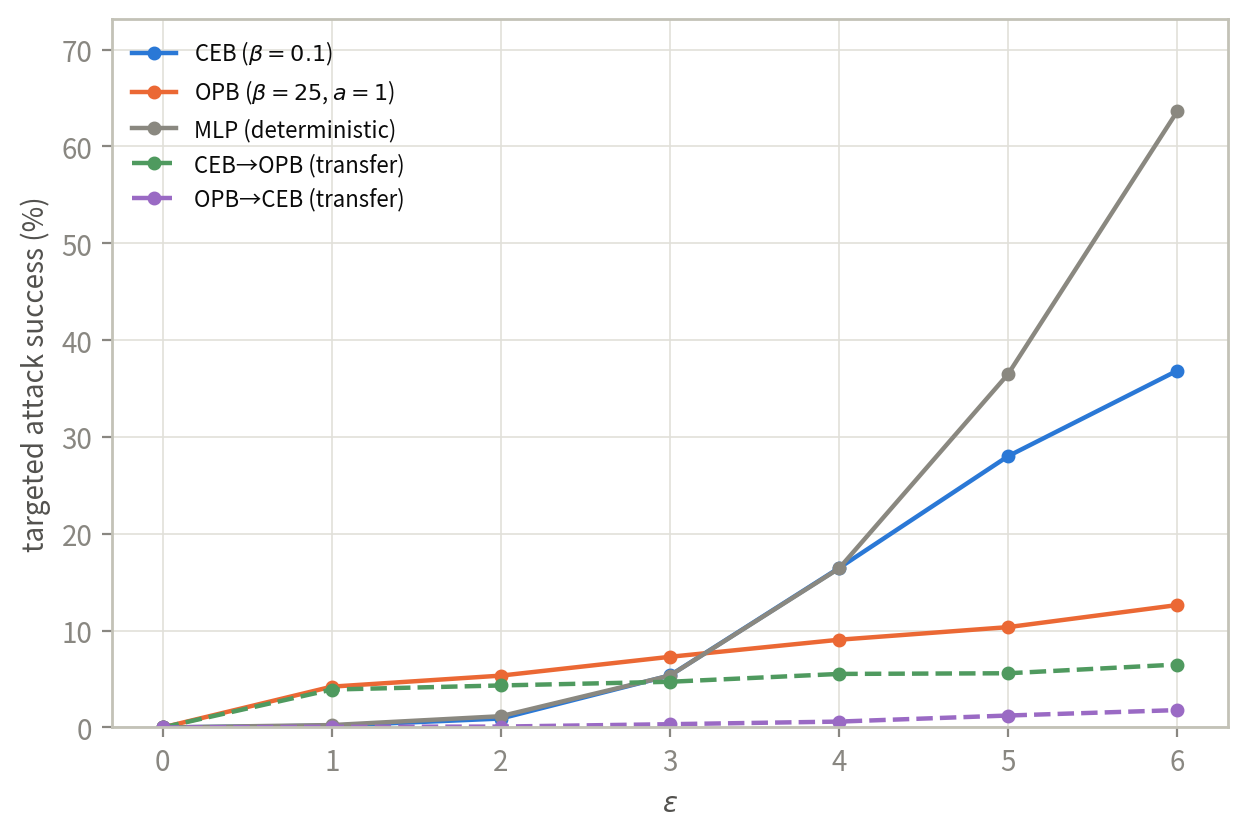
\includegraphics[width=0.48\linewidth]{figures/fig_adv_transfer_l2_mnist.png}
\caption{Transfer PGD curves on MNIST (gradient-masking check). Targeted adversaries
are generated on one model and evaluated on another; CEB-to-OPB transfer remains far
below OPB's own white-box attack. The targeted white-box curves are in the main text.}
\label{fig:adv-transfer}
\end{figure*}
